\documentclass{beamer}
\usepackage{xcolor}
\usepackage{hyperref}
\usepackage{perpage} 	% Numeroter footnote par page
\usepackage{fontawesome5}
\MakePerPage{footnote}
\usetheme{Singapore}
\title[Accord All Staff Meeting]{Towards a Portable Model for All-scale Predictions}

\subtitle{Accord All Staff Meeting}

\author{Loïc Maurin, Fabrice Voitus}

\institute[CNRM]{Centre National de Recherche Météorologique}

\date{April 18th, 2024}
\titlegraphic{
    
\includegraphics[height=1cm]{png/logos/logo_cnrm.jpg}
    
\includegraphics[height=1cm]{png/logos/logo-mf-blanc-fond-bleu-baseline-jpeg.jpg}
}
\AtBeginSection[]
{
  \begin{frame}{Table of contents}
      \tableofcontents[currentsection]
  \end{frame}
}
\renewcommand{\arraystretch}{1.5}
\addtobeamertemplate{navigation symbols}{}{%
    \usebeamerfont{footline}%
    \usebeamercolor[fg]{footline}%
    \hspace{1em}%
    \insertframenumber/\inserttotalframenumber
}
\setbeamercolor{footline}{fg=blue}
\setbeamerfont{footline}{series=\bfseries}
\setbeamertemplate{caption}[numbered]
%%%%%%%%%%%%%%%%%%%%%%%
\begin{document}
\frame{\titlepage}

%%%%%%%%%%%%%
\begin{frame}{Table of contents}
    \tableofcontents
\end{frame}

\section{Introduction}
%%%%%%%%%%%%%
\begin{frame}{A dynamical core for very-high resolution NWP applications}

    \begin{block}{Objectives}
        \begin{itemize}
            \item[\faIcon{mountain}] Improving stability over steep orography
            \item[\faIcon{laptop-code}] Maintaining scalability over massively parallel HPC-clusters
        \end{itemize}
    \end{block}

\end{frame}

\begin{frame}{Current status of AROME perfomances}

\end{frame}

\begin{frame}{AROME and FVM dynamical cores - Summary}
    \begin{center}
        \resizebox{\textwidth}{!}{
        \begin{tabular}{|c|c|c|}
            \hline
              & AROME & FVM \\
            \hline
            Vertical coordinate & Mass-based & Height-based  \\
            \hline
            Discretization & Spectral Transform (ST) & Finite Volumes (FV)\\
            \hline
            Linearization & Constant Coefficients & Non-constant Coef. (NC) \\
            \hline
            Implicit solver & Direct & Krylov Methods \\
            \hline 
            Advection & Semi-Lagrangian (SL) & Eulerian (MPDATA)\\
            \hline 
        \end{tabular}
        }
    \end{center}
\end{frame}

\begin{frame}{PMAP - FVM dynamical core}

    \begin{block}{Finite Volume Module (FVM)}
        \begin{itemize}
            \item Eulerian non-oscillatory flux-form advection : MPDATA
            \item 2 time levels semi-implicit integration \newline\tiny \textit{(implicit treatment of acoustic, 
            buoyant modes and metric terms for orography)}
            \normalsize \item Height-based terrain-following coordinate
        \end{itemize}
    \end{block}

    \begin{block}{MPDATA -  \scriptsize \textit{Multi Dimensional Positive Definite Advection Transport Algorithm}}
       
        \begin{itemize}
            \item Conservative transport scheme
            \item Conditional stability with $CFL < 0.5$ (implies small time steps)
        \end{itemize}
        
    \end{block}

\end{frame}


% \section{Components}
\begin{frame}{Vertical coordinate}
    \begin{block}{Mass-based}
        \begin{itemize}
            \item[\textcolor{blue}{\faIcon{plus}}] \small Hydrostatic part of the flow given by the coordinate
            \item[\textcolor{blue}{\faIcon{plus}}] \small  Reduced need for a top absorbing layer ($z \rightarrow \infty$) 
            \item[\textcolor{red}{\faIcon{minus}}] \small Time dependency of metric terms ($\pi_s = \pi_s(x, y, t)$)
            \item[\textcolor{red}{\faIcon{minus}}] \small Integral vertical operators
        \end{itemize}
    \end{block}

    \begin{block}{Height-based}
        \begin{itemize}
            \item[\textcolor{blue}{\faIcon{plus}}] \small Metric terms (orography) independant for the time
            \item[\textcolor{red}{\faIcon{minus}}] \small Top absorbing layer required 
            \item[\textcolor{red}{\faIcon{minus}}] \small Dependency to a prescribed hydrostatic ambient state
        \end{itemize}
    \end{block}
\end{frame}

\begin{frame}{Solver : improving stability over steep orography}

    \textcolor{red}{Inclusion of metric terms for orography in the implicit solver}
    
    \begin{block}{AROME - Constant Coefficients}

        \begin{itemize}
            \item[\textcolor{red}{\faIcon{minus}}] \small Instabilities on steep slopes ($>$ 60°)

            \item \textcolor{blue}{Direct Spectral solver}
            \begin{itemize}
                \item[\textcolor{blue}{\faIcon{plus}}] \small  Exact solution in a single iteration 
                \item[\textcolor{red}{\faIcon{minus}}] \small  Non-constant coefficient computationnally intractable 
            \end{itemize}
            \item \textcolor{blue}{Iterative solver}
            \begin{itemize}
                \item[\textcolor{blue}{\faIcon{plus}}] \small Fixed number of iterations for the implicit solver
                \item[\textcolor{blue}{\faIcon{plus}}] \small Near-constant weak scalability while increasing the resolution
            \end{itemize}
        \end{itemize}
        
    \end{block}

    \begin{block}{FVM - Non-constant Coefficients - Iterative solver}
        \begin{itemize}
            \item[\textcolor{blue}{\faIcon{plus}}] \small Stable on steep slopes (up to 85°) 
            \item[\textcolor{red}{\faIcon{minus}}] \small Convergence rate depends on the prescribed ambient state
        \end{itemize}
    \end{block}
\end{frame}

\begin{frame}{Zängl experiment with FVM}
    \begin{figure}
        \centering
        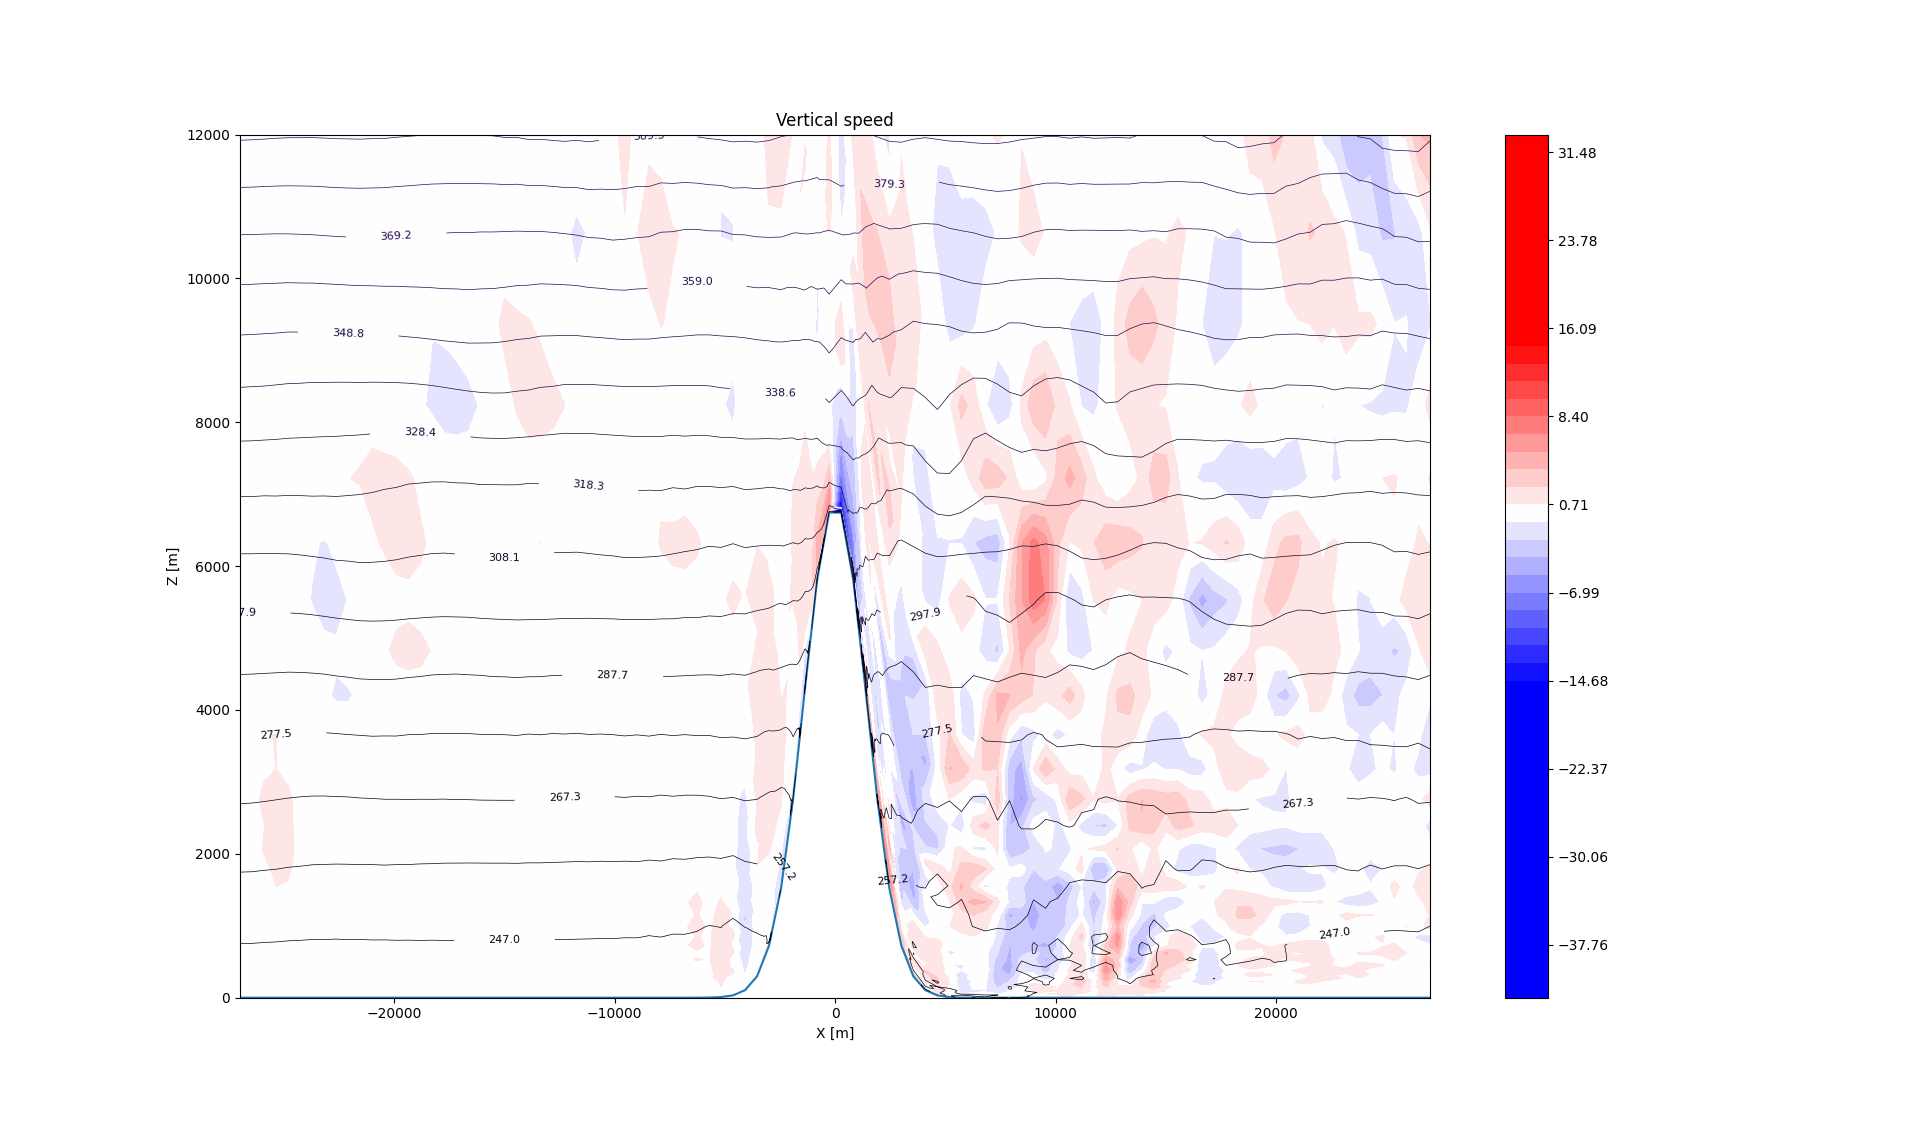
\includegraphics[scale=0.2]{png/zangl_isothermal.png}
        \caption{Zängl experiment with FVM : prescription of an uniform horizontal wind 
        speed $u = 20$ $m.s^{-1}$ and isothermal conditions on a gaussian shape. The maximum slope 
        is $75^{\circ}$. Results after 6 hours with a time step $\delta t_{run} = 0.10$ $s$.  }
        \label{fig:zangl}
    \end{figure}

\end{frame}



\begin{frame}{Solver : improving numerical efficiency}

    \begin{columns}
        \column{0.5\textwidth}
        \begin{block}{Direct spectral solver}
            \begin{itemize}
                \item[\textcolor{blue}{\faIcon{plus}}] Exact solver (no iterations)
                \item[\textcolor{red}{\faIcon{minus}}] Global communications for Spectral Transform 
            \end{itemize}
        \end{block}
    
        \begin{block}{Iterative Krylov solver}
            \begin{itemize}
                \item[\textcolor{blue}{\faIcon{plus}}] Near constant weak scalability
                \item[\textcolor{red}{\faIcon{minus}}] Convergence rate
            \end{itemize}
        \end{block}

        % \textcolor{red}{Investigating a Multigrid preconditioner}

        \column{0.5\textwidth}
        \begin{figure}
            \centering
            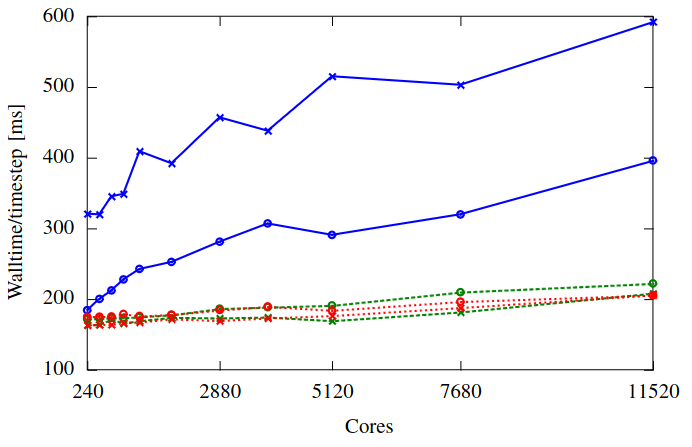
\includegraphics[scale=0.25]{png/weak_scalability_beaufix.png}
            \caption{\footnotesize  Weak scalability experiments on : spectral solver (\textcolor{blue}{solid blue}), GCR(k) (\textcolor{green}{dashed green}), 
            Richardson (\textcolor{red}{short-dashed red})}
            \label{fig:evolution_chaotique}
        \end{figure}
    \end{columns}

    \tiny Degrauwe D, Voitus F, Termonia Piet. A non-spectral Helmholtz solver for numerical weather prediction models with a mass-based vertical coordinate. QJR Meteorol. Soc. 2020; 1-15. 

\end{frame}


\begin{frame}{Transport scheme : Semi-Lagrangian vs. Eulerian MPDATA}
    
    \begin{block}{MPDATA}
        \begin{itemize}
            \item[\textcolor{blue}{\faIcon{plus}}] Conservative scheme
            \item[\textcolor{blue}{\faIcon{plus}}] Non-oscillatory 
            \item[\textcolor{red}{\faIcon{minus}}] Conditionnally stable ($CFL < 0.5$)
        \end{itemize}
    \end{block}

    \begin{block}{Pointwise Semi-Lagrangian scheme}
        \begin{itemize} 
            \item[\textcolor{blue}{\faIcon{plus}}] Unconditionnally stable
            \item[\textcolor{blue}{\faIcon{plus}}] Performs well with CFL between 4 and 10
            \item[\textcolor{red}{\faIcon{minus}}] Non conservative under strong deformations
        \end{itemize}
    \end{block}
    
\end{frame}

\begin{frame}{Transport scheme : Semi-Lagrangian vs. Eulerian MPDATA}
    Semi-Lagrangian Advection
    \begin{figure}
        \centering
        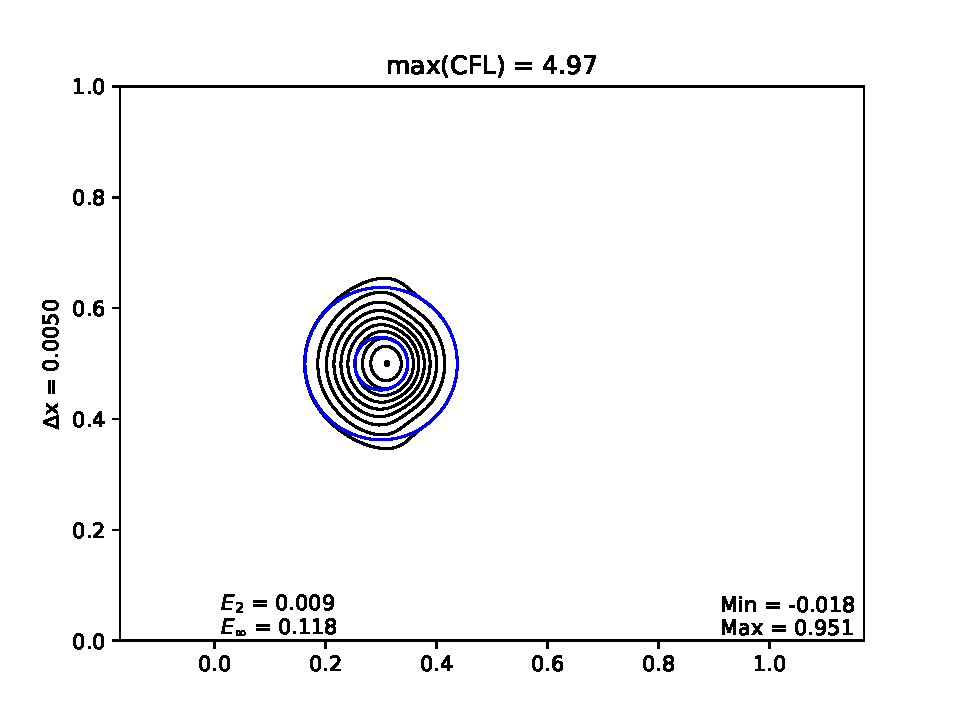
\includegraphics[scale=0.5]{png/blossey_sl_005_unfiltered.pdf}
        \caption{Durran and Blossey advection test with Semi-Lagrangian Algorithm : $CFL_{max} = 4$}
        \label{fig:blossey}
    \end{figure}
\end{frame}





%%%%%%%%%%
% \section{First Experiments on FVM}

% \begin{frame}{No flow over a gaussian orography}
%     \begin{figure}
%         \centering
%         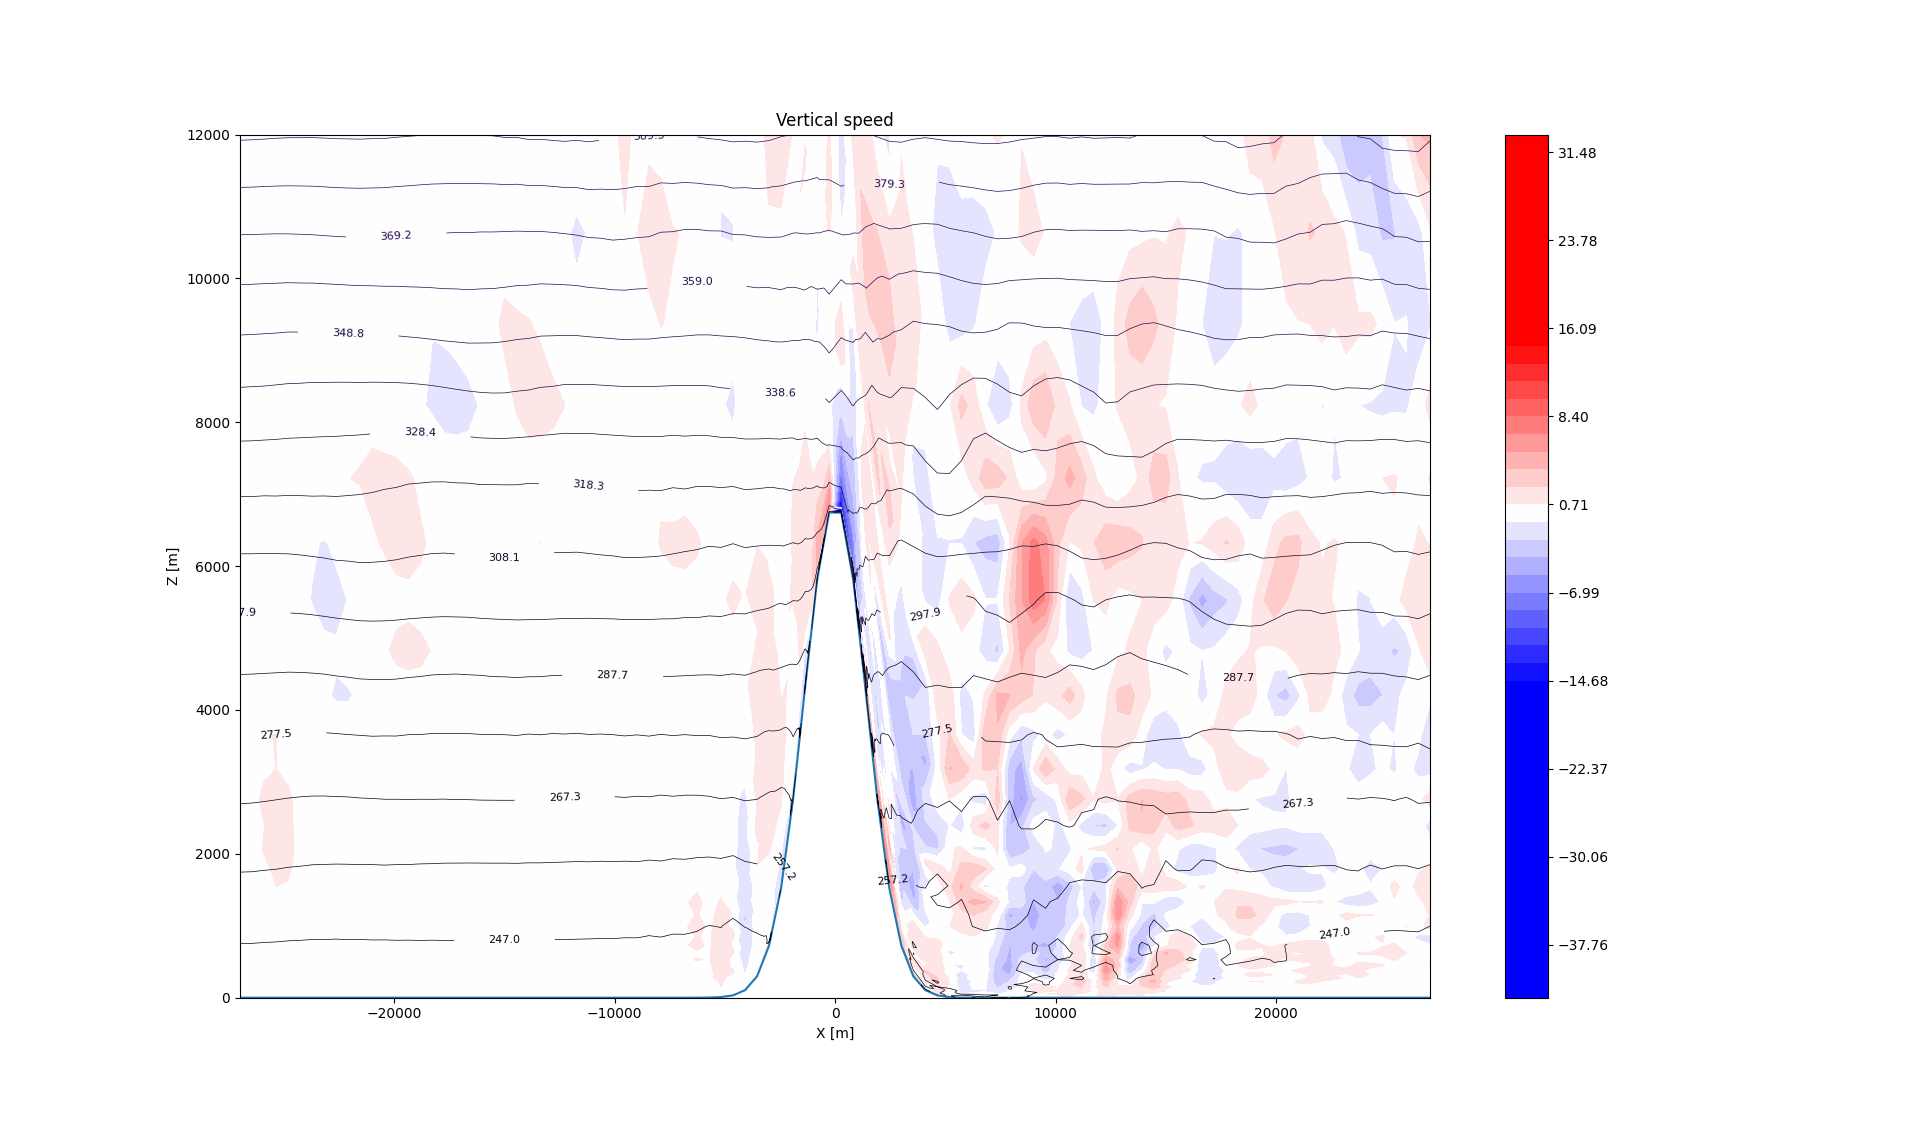
\includegraphics[scale=0.2]{png/zangl_isothermal.png}
%         \caption{Reproduction of Zängl experiment : prescription of an uniform horizontal wind 
%         speed $u = 20$ $m.s^{-1}$ and isothermal conditions on a gaussian shape. The maximum slope 
%         is $75^{\circ}$. Results after 6 hours with a time step $\delta t_{run} = 0.10$ $s$.  }
%         \label{fig:zangl}
%     \end{figure}
% \end{frame}

\begin{frame}{Uniform flow over a steep orography on a vertical plane}

    \begin{center}
        \begin{tabular}{|c|c|c|c|c|}
            \hline
              Maximum slope & $CFL_{max}$ & $Lipschitz$ & $\Delta t$ & $\Delta z_{min}$\\
            \hline
            $15^{\circ}$ & 0.5 &  &  3 &  10 \\
            \hline
            % $30^{\circ}$ &  &  &  & 10 \\
            % \hline
            $45^{\circ}$ &  &  &  & 10 \\
            \hline
            % $60^{\circ}$ &  &  &  & 10 \\
            % \hline 
            $75^{\circ}$ &  &  &  & 10 \\
            \hline 
        \end{tabular}       
    \end{center}

    \begin{block}{Lipschitz' condition for Semi-Lagrangian convergence} 
        $L = max(\delta t \lvert \frac{\partial u}{\partial x} \rvert, \delta t \lvert \frac{\partial v}{\partial y} \rvert, \delta t \lvert \frac{\partial w}{\partial z} \rvert)$
    \end{block}

\end{frame}

% \begin{frame}{No flow over the Alps}

%     \begin{figure}
%         \centering
%         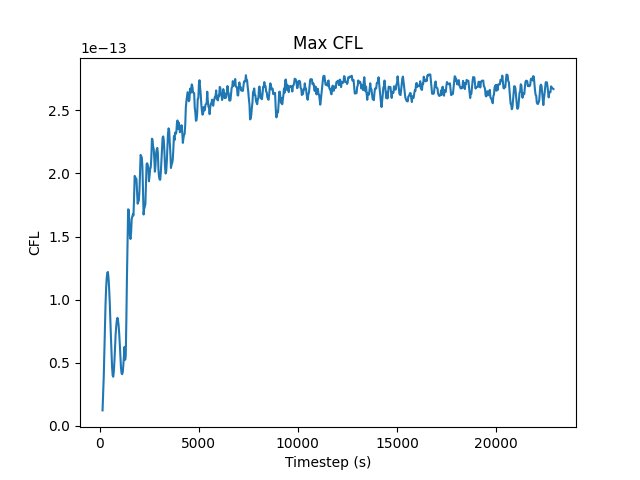
\includegraphics[scale=0.4]{png/no_flow_alps_max_cfl.png}
%         \caption{Maximum advective CFL for a run over an Alpine domain. Domain imported from AROME, 
%         with an horizontal resolution of 0.25° (1,25 km), $\delta z_{min} = 8m$, 
%         maximum slope : $35°$. Run over 6 hours. $\delta t = 30 s$.}
%         \label{fig:domaine_arome}
%     \end{figure}
    
% \end{frame}

%%%%%%%%%%%
\section{Towards a Demonstrator}

\begin{frame}{Physical processes for PMAP-FVM}

\begin{block}{Coupling ICE3 Microphysics scheme to FVM}
    \begin{itemize}
        \item \small Translation of ICE3 to GT4Py
        \item Coupling of ICE3 and FVM with respect to small time steps options (Méso-NH)
    \end{itemize}
\end{block}

% \begin{block}{Coupling physics schemes}
%     \begin{itemize}
%         \item \small Radiations scheme ecRad translated by ETHZ
%         \item Surface scheme
%     \end{itemize}
% \end{block}

\end{frame}

\begin{frame}{Building on GT4Py + DaCe}

\begin{block}{GT4Py : GridTools for Python}
    \begin{itemize}
        \item \small Domain System Language (DSL) for HPC code generation
        \item \small Portable accross CPU and GPU architectures
        \item[\faPython] \small Python code : readability and Object Oriented Programming
    \end{itemize}    
\end{block}

\begin{block}{DaCe : Data Centric Parallel Programming}
    \begin{itemize}
        \item \small Optimizing memory allocation for stencils
        \item \small DaCeML : Merging AI and Physics based models
        \begin{itemize}
            \item \small Model inference using ONNX and integration with Pytorch
            \item \small Automatic differenciation engine
        \end{itemize}
    \end{itemize}
\end{block}
\end{frame}


%%%%%%%%%%%
\section{Future work}
\begin{frame}{Building a demonstrator with PMAP}
    \textcolor{red}{Development of a realistic model for Limited Area and LES}

    \begin{block}{Physics packages on GT4Py}
        \begin{itemize}
            \item Integration of GT4Py physics package to PMAP
            \begin{itemize}
                \item[\faCloudShowersHeavy] \small ICE3 - Microphysics + Adjustments
                \item[\faIcon{radiation}] ecRad (translated by ETHZ)
                \item[\faWind] Turbulence scheme from COSMO
            \end{itemize}
            \item Translation of packages 
            \begin{itemize}
                \item \small SURFEX
                \item Shallow Convection
            \end{itemize}
        \end{itemize}
    \end{block}

    % \begin{block}{Towards realistic runs}
    %     \begin{itemize}
    %         \item Investigation of
    %     \end{itemize}
    % \end{block}

\end{frame}

\end{document}